\documentclass{book}
\usepackage{graphicx}
\usepackage{color}
\usepackage{url}
\usepackage{amssymb}
\usepackage{appendix}
\usepackage[hidelinks]{hyperref}
\usepackage{fontspec}	% To change default font
%\usepackage{fancyhdr}	%to include customized footer and header
%\pagestyle{fancy}
%\lhead{}
%\chead{\leftmark}
\graphicspath{{./Figures/}}
\setmainfont{URW Palladio L} % Use if font is to be set

\begin{document}
%-----------------------------------
% For customised Title Page
\thispagestyle{empty}
%\input{./title.tex} %Cover page
\thispagestyle{empty}
%\input{./inner.tex}	%Inner title page
%--------------------------------------------------------------------

%Default Title page 
\title{Analog Communication
Laboratory Manual}
\date{December 2013}
\author {Authors: Kavya Manohar, Contributor-2...}
\maketitle
%----------------------------------------------------------
%\thispagestyle{empty}
  
\textcopyright{}2013
\\[5cm]
    This work is licensed under a Creative Commons Attribution-Share Alike 4.0 India License. See \url{http://creativecommons.org/licenses/by-sa/4.0/} for more details.
%------------------------------------------------------------






\thispagestyle{empty}
\tableofcontents
\thispagestyle{empty}
\thispagestyle{empty}

\listoffigures
\thispagestyle{empty}
%CHAPTER-----------------------------------------------------------------------

\chapter [Introduction to Analog Communication]{Introduction to Analog Communication}


\cite{ACmanual}Communication is the transfer of information from one place to another. A bidirectional communication system operates in opposite directions. The receiver can respond
to the sender. Radio communication uses electrical energy to transmit information. Because electrical energy travels almost as fast as light, radio communication is essentially instantaneous.
A radio transmitter converts audio (sound) signals to electrical signals that are sent over wires or through space. A radio receiver converts the electromagnetic waves back to sound waves so that the
information can be understood. 

The transmitted information is the \textbf {intelligence signal} or \textbf{ message signal}.
 Message signals are in the \textbf {Audio Frequency (AF)} range of low frequencies from about 20 Hz to 20 kHz.
 
 
The \textbf{Radio Frequency (RF)}  is the carrier signal. Carrier signals have high frequencies that range from 10 kHz up to about 1000 GHz.
A radio transmitter sends the low frequency message signal at the higher carrier signal frequency by combining the message signal with the carrier signal.

\textbf{Modulation} is the process of changing a characteristic of the carrier signal with the message
signal. In the transmitter, the message signal modulates the carrier signal.
The modulated carrier signal is sent to the receiver where \textbf{demodulation} of the carrier occurs to
recover the message signal.\\[10pt]
\textsc{\textbf {IMPORTANT TERMS}}
\begin{itemize}
\item \textbf{Audio} - signals that a person can hear.

\item \textbf{Electromagnetic waves} - the radiant energy produced by oscillation of an electric
charge.

\item \textbf{Intelligence signal} - any signal that contains information; it is also called the
message signal.
\item \textbf{Message signal} - any signal that contains information; it is also called
the intelligence signal. 
\item \textbf{Audio Frequency (AF)} - frequencies that a person can hear.
AF signals range from about 20 Hz to 20 kHz.
\item \textbf{Radio Frequency (RF)} - the transmission frequency of electromagnetic (radio) signals.
RF frequencies are from about 300 kHz to the 1,000,000 kHz range.
\item \textbf{Carrier signal} - a single, high-frequency signal that can be modulated by a message
signal and transmitted.
\item \textbf{Modulation} - the process of combining the message signal with the carrier signal that
causes the message signal to vary a characteristic of the carrier signal.
\item \textbf{Demodulation} - the process of recovering or detecting the message signal from the
modulated carrier frequency.
\item \textbf{Amplitude Modulation (AM)} - the process of combining the message signal with
the carrier signal and the two sidebands: the lower sideband and the upper
sideband.
\item \textbf{Frequency Modulation (FM)} - the process of combining the message signal with
the carrier signal that causes the message signal to vary the frequency of the
carrier signal.
\item \textbf{Phase Modulation (PM)} - the process of combining the message signal with the
carrier signal that causes the message signal to vary the phase of the carrier signal.
\item \textbf{Angle modulation} - the process of combining the message signal with the carrier signal that causes the message signal to vary the frequency and/or phase of the
carrier signal.
\item \textbf{Balanced modulator} - an amplitude modulator that can be adjusted to control the
amount of modulation.
\item \textbf{Double-Sideband (DSB)} - an amplitude modulated signal in which the carrier is
suppressed, leaving only the two sidebands: the lower sideband and the upper
sideband.
\item \textbf{Mixer}- an electronic circuit that combines two frequencies.
\item \textbf{Product detector} - a detector whose audio frequency output is equal to the product of the
Beat
Frequency Oscillator (BFO) and the RF signal inputs.
\item \textbf{Phase detector} - an electronic circuit whose output varies with the phase differential
of the two input signals.
\item \textbf{Envelopes}- the waveform of the amplitude variations of an amplitude modulated
signal. 
\item \textbf{Sidebands} - the frequency bands on each side of the carrier frequency that
are formed during modulation; the sideband frequencies contain the intelligence of
the message signal.
\item \textbf{AM} - an amplitude modulated signal that contains the carrier signal and the two
sidebands: the lower sideband and the upper sideband.
\item \textbf{Bandwidth} - the frequency range, in hertz (Hz), between the upper and lower
frequency limits. 
\item \textbf{Harmonics} - signals with frequencies that are an integral multiple of
the fundamental frequency. 
\item \textbf{Beat Frequency Oscillator (BFO)} - an oscillator whose
output frequency is approximately equal to the transmitter's carrier frequency and is
input to a product detector
\end {itemize}

\chapter[Tuned Amplifier using IFT]{Tuned Amplifier using IFT}
\label{iftamplifier}
%-------------------
\section*{Aim}
To design and implement a tuned frequency amplifier using BJT and IFT.
%--------------------
\section*{Theory}


Intermediate frequency amplifiers are tuned voltage amplifiers used to amplify a particular frequency. Its primary function is to amplify only the tuned frequency with maximum gain and reject all other frequencies above and below this frequency. This type of amplifiers are widely used in intermediate frequency amplifiers in AM super heterodyne receivers, where intermediate frequency is usually 455 kHz.

In common emitter voltage amplifier circuit (emitter bypassed), the voltage gain is $A_V=\frac{R_C||R_L}{r_e}$, where $R_C$ is the collector resistance in the circuit, $R_L$ is the load resistance and $r_e$ is the internal emitter resistance. In tuned voltage amplifier the collector resistance is replace by a tuned load upon which  the gain is dependant. For a parallel resonating circuit cosisting of a capacitor, C and an inductor,L the impedance $Z_o$ is maximum at resonant frequency, $f_o=\frac{1}{2\pi \sqrt{LC}}$. So an amplifier with tuned load will have maximum gain at resonant frequency.
In practical tuned amplifier circuits, an intermediate frequency transformer(IFT) is used as tuned load. IFT is tuned to standard 455 kHz audio frequency, (See \ref{IFT}).

The quality factor of the circuit is given by $Q=\frac{f_o}{Bandwidth}$.

\section*{Design}
Inorder to design a common emitter amplifier operating at high frequency, one can use a high frequency transistor like BF194, BF195, BF494, BF495 or 2N2222.
\\Choose transistor BF 194/195. For its datasheet See \ref{BF194/195},\\


\noindent Let $V_{CC}$ be 10\% more than the required output amplitude, ie. 10V.
\begin{equation}
\therefore V_{CC}=12\ V
\end{equation}
\begin{equation}
I_c<10 \% \ of \  I_{Cmax} =\ 10\%\  of\  30\  mA =\ 3 mA
\end{equation}
\noindent Let $I_c=\ 1 mA$.
%\noindent The current gain,
%\begin{equation}
%h_{FEmin}=\ 67
%\end{equation}
Let the stability factor of the circuit be,
\begin{equation}
S=10
\end{equation}

\noindent Under dc  conditions, the primary dc resistance of the IFT is very small($<5\Omega$). So dc voltage drop across collector circuit is very low, approximately zero.

\noindent For class A mode of operation set, 
\begin{equation}
 V_{CE} = \frac{V_{CC}}{2}= 6 V
\end{equation}
\paragraph{Design of Emitter resistance}
\noindent \\The voltage across emitter resistance is,
\begin{equation}
V_{RE}=V_{CC}- V_{CE} =\ 12V-\ 6V=\ 6V
\end{equation}
\begin{equation}
I_E \approx I_C 
 \end{equation}
\noindent Hence
\begin{equation}
I_E = 1mA
\end{equation}
\noindent Thus
\begin{equation}
R_E=\ \frac{V_{RE}}{I_E}=\ \frac{6V}{1mA}=\ 6k\Omega
\end{equation}
\noindent Choose standard value of $R_E=\ 5.6 \ k\Omega$.
\paragraph{Design of Potential divider biasing\\}
\noindent The Stability factor S=10. Assuming $R_B$ is the effective resistance at the base,
\begin{equation}
S=\ 10=\ 1+\frac{R_B}{R_E}
\end{equation}
\begin{equation}
R_B=\ 9R_E=\ 50.4k\Omega
\end{equation}
\begin{equation}
\label{R1R2}
R_B=\ R_1||R_2=\ \frac{R_1R_2}{R_1+R_2}=\ 50.4k\Omega
\end{equation}
\noindent The voltage at the base of the transistor is 
\begin{equation}
V_B=\ V_E+\ V_{BE}=\ V_{RE}+\ V_{BE}=\ 6V+\ 0.6V=\ 6.6 V
\end{equation}

\noindent This is the voltage across $R_1$. 
\begin{equation}
V_{R1}= V_{CC} \frac{R_2}{R_1+R_2}=\ 6.6V
\end{equation}

\begin{equation}
\label{R2}
\frac{R_2}{R_1+R_2}=\ \frac{6.6V}{12V}=\ 0.55
\end{equation}
From equations \ref{R1R2} and \ref{R2}, 
\begin{equation}
R_1=\ 91.4\ k\Omega \approx \ 82\ k\Omega \ and \ R_2=100\ k\Omega
\end{equation}
\noindent Choose load resistor as 
\begin{equation}
R_L=\ 100 k\Omega
\end{equation}
\subsubsection{Design of capacitors}
\noindent The capacitors $C_1$, $C_2$  and $C_E$  can be designed based on lower cut-off frequency at -3 dB point. Since this frequency is much lower than 300 kHz, Choose low values of capacitance like \begin{equation}
C_1=\ C_2=\ C_E=\ 1 \ \mu F
\end{equation}

\section*{Circuit Diagram}
See Figure \ref{IFTuned} for circuit diagram.
\begin{figure}[ht]
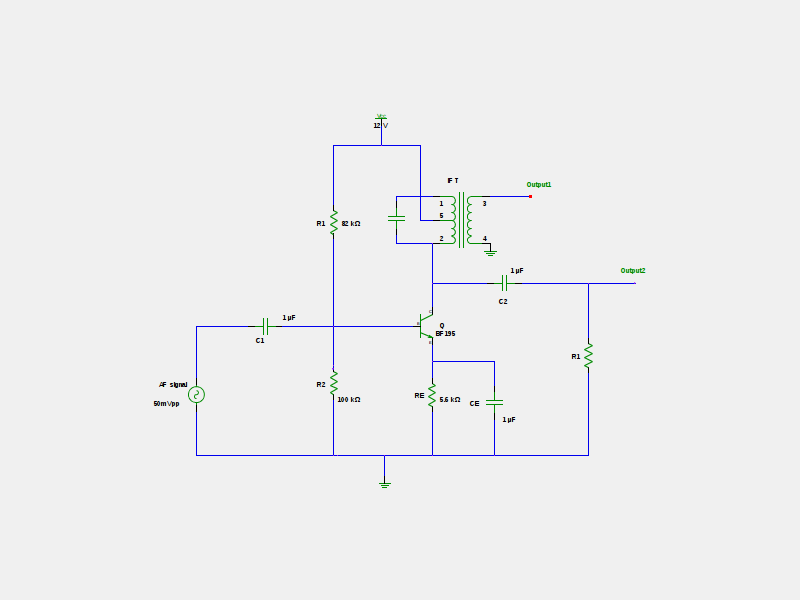
\includegraphics[width=12cm, height=8cm, trim=2cm 3.5cm 5cm 3.5cm,clip=true]{IFTuned.png}
\caption{Circuit Diagram for IF Tuned Amplifier}
\label{IFTuned}
\end{figure}
\section*{Procedure}
\begin{itemize}
\item
Assemble the circuit as shown in the circuit diagram.
\item
Obtain output from output-1 or output-2 terminal as in the circuit diagram.
\item
Give input signal, which is a sinewave of frequency variable from 300 kHz to 600 kHz and amplitude 50 $mV_{pp}$.
\item
Observe the output waveform on a CRO. 
\item
Enter the details of input and output waveforms on the tabular column shown.
\item
Calculate gain $A_V$ by varying $f_{in}$.($A_V= \ \frac{V_{outpp}}{V_{inpp}}$)

\item
Plot frequency response characteristics with $f_{in} (kHz) $ along x-axis and  $Gain_{dB}=\ 20\ log\ A_v$ along y-axis.
\item
Find the resonant frequency, 3-dB bandwidth and hence the Q-factor.
\end{itemize}
\section*{Observation}
\begin{center}

\begin{tabular}{|l|l|l|l|l|}

\hline
  & & & &\\
 
$f_{in} (kHz) $  & $log_{10}\ f_{in}$  &  $V_{outpp}(V)$ & $A_v\ =\frac{V_{outpp}}{V_{inpp}} $ & $Gain_{dB}=\ 20\ log\ A_v$ \\ \hline
 & & & &\\ \hline
& & & &\\ \hline
& & & &\\ \hline
& & & &\\ \hline
& & & &\\ \hline
& & & &\\ \hline

\end{tabular}
\end{center}
%\textcolor{red}{TODO:frequency response curve of gain to be added}. 
\section*{Result}
A tuned amplifier was implemented using IFT.\\
Its maximum gain= \\
Resonant frequency, $f_0$= \\
Band-width, $BW$ =\\
Q-factor=$\frac{f_0}{BW}$

\chapter[Amplitude Modulation- Generation]{Amplitude Modulation- Generation}

\section*{Aim}
To design and set-up  an AM generator using BJT and measure the modulation index from the observed output waveform.

\section*{Theory}
\paragraph{}
	The transistor $T_1$ is configured as a common emitter amplifier. The RF carrier wave is given at the base through a coupling capacitor $C_1$.  The message signal used for modulation is the AF signal applied between the emitter resistance and the ground. The message signal modulates the envelope of the carrier which is obtained as output from the collector through a coupling capacitor $C_3$. 
\paragraph{}
The ratio of the maximum amplitude of the modulating signal voltage to that of the carrier voltage is termed as modulation index. This is represented as $m=\frac{V_m}{V_c}$.


\section*{Design}
\textcolor{red}{Design steps need to be verified}

\paragraph{DC Biasing conditions:}
Choose BF194 which is a high frequency transistor. From its datasheet (See \ref{BF194/195}) the various parameters can be obtained as:

 
Let the supply voltage be 60\% of the maximum $V_{ce}$.  \begin{equation}
V_{cc}=\ 60\% of V_{cemax}=\ 12 V
\end{equation}

\noindent Let the collector current $I_c$ be 10\% of maximum rated value.
\begin{equation}
I_{c}=\ 3\% \ of \ I_{cmax}=\ 1 mA
\end{equation}

\noindent In-order to fix the biasing point in the middle of load line, let $V_{RC}$ be 40\% of $V_{cc}$, $V_{RE}$\ be\ 10\% \ of $V_{cc}$ and $V_{ce}$\  be\ 50\% \ of $V_{cc}$.
\begin{equation}
V_{RC}=\ 45\% \ of \ V_{cc}=\ 5.4V
\end{equation}
\begin{equation}
V_{RE}=\ 5\% \ of \ V_{cc}=\ 0.6V
\end{equation}
\begin{equation}
V_{ce}=\ 50\% \ of \ V_{cc}=\ 6V
\end{equation}
\paragraph{Design of Resistors:}
\begin{equation}
R_C=\frac{V_{RC}}{I_c}=\ \frac{5.4V}{1mA}=\ 5.4 k\Omega
\end{equation}
\begin{equation}
R_E=\frac{V_{RE}}{I_e}=\ \frac{0.6V}{1mA}=\ 600\Omega
\end{equation}
\noindent From the datasheet, hFE has a minium value of 67. 
\begin{equation}
I_b=\frac{I_c}{hFE}=\frac{1mA}{67}=\ 15 \mu A
\end{equation}
\noindent Assume the current through $R_1=\ 10 I_b$ and that through $R_2=9I_b$ 
\begin{equation}
 V_{R2}=V_{be}+V_{RE}\\ =0.7+0.6V=1.3V
\end{equation}
\noindent Then
\begin{equation}
R_2=\frac{V_{R2}}{9I_b}=\frac{1.2V}{9X15X10^{-6}}=8.8 k\Omega
\end{equation}
\noindent and 
\begin{equation}
R_1=\frac{V_{R1}}{10I_b}=\frac{10.8V}{10X15X10{^-6}}= 72k\Omega
\end{equation}

\noindent Based on these design equations use the standard resistor values of $R_1=22k\Omega,\ R_2=10k\Omega, \ R_c=10k\Omega,\ R_c=560\Omega$ and a load resistance of $R_L=1k\Omega$.
Use coupling capacitors $C_1=0.1 \mu F,\ C_2=0.001\mu F$ and emitter bye-pass capacitor $C_E=0.01\mu F$.
\section*{Components and Equipments Required}
Function Generators(2), CRO(2), Connection wires, Breadboard, Probes.
\\BF194 - High frequency bipolar junction transistor
\\ $22k\Omega,\  10k\Omega\ (2),\ 560\Omega,\,\ 1k\Omega $ - Resistors
\\ $ 0.1\mu F,\ 0.01\mu F, \ 0.001\mu F $ - Capacitors
\\ 
\section*{Circuit Diagram}
\begin{figure}[h]
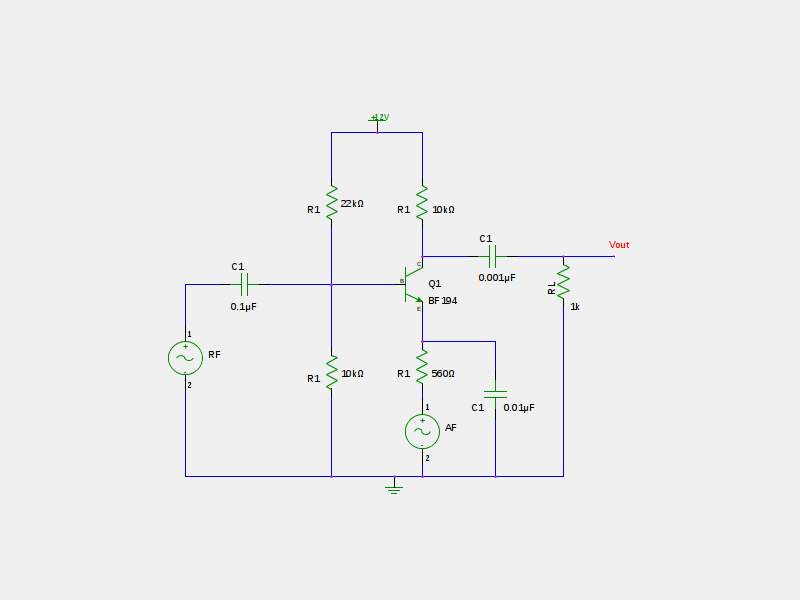
\includegraphics[width=15cm, height=10cm, trim=5cm 3.5cm 4cm 3.5cm, clip=true]{AM.png}
\caption{Circuit Diagram for Amplitude modulation using BJT}

\end{figure}

\section*{Procedure}
\begin{enumerate}
\item
Set up the circuit after verifying the condition of components.
\item
Feed AF modulating signal (say, $f_m=1kHz$ and $E_m=150mV$) and Rf carrier (say, $f_c=70kHz$ and $E_c=300mV$) using function generators.
\item
Adjust amplitude and frequencies of the AF and RF signals and observe amplitude modulated waveform on the CRO.
\item
Fix $f_m$ and $f_c$. Note down $E_{max}$ and $E_{min}$ of the AM signal and calculate modulation index according to the formula ,
\begin{equation}
m=\frac{E_{max}-E_{min}}{E_{max}+E_{min}}.
\end{equation}
Here $E_{max}$ is the maximum of the positive envelope of the carrier and $E_{min}$ is the minimum of the positivee envelope of the carrier.
\item
Repeat for different values of $E_m$ and $E_c$. Observe the AM waveforms for different values of m.
\item
Plot the waveforms on a graph sheet.
\item

Fill in the observation column
\end{enumerate}


\section*{Observation}


\begin{figure}[h]

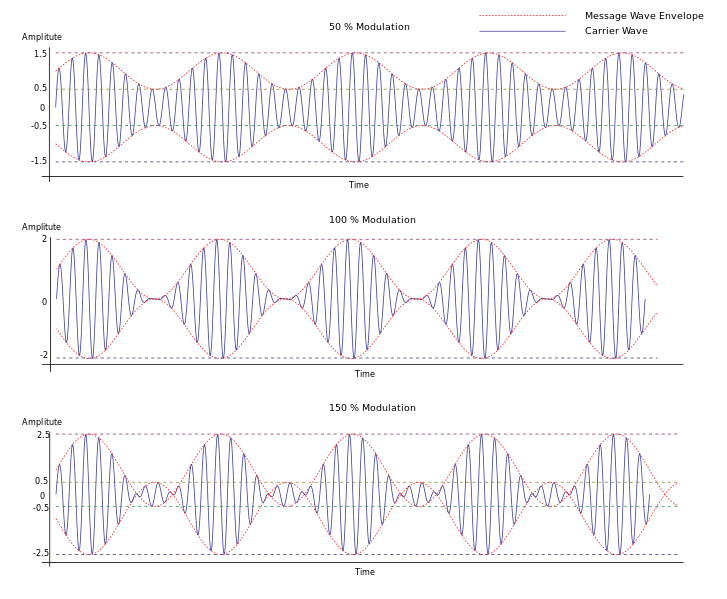
\includegraphics[width=\textwidth]{AMmodindex.png}
\caption{Effect of modulation index on AM}
\label{AMmodindex}
\end{figure}
\noindent Fig \ref{AMmodindex}  shows the effect of modulation index on the resultant AM wave\footnote{\url{https://commons.wikimedia.org:/wiki/File:Amplitude_Modulated_Wave-hm-64.svg}}
\begin{center}

\begin{tabular}{|l|l|l|}

\hline
 & &\\
 
$E_{min}$  & $E_{max}$ & $m=\frac{E_{max}-E_{min}}{E_{max}+E_{min}}$ \\
 & & \\ \hline
 & & \\ \hline
& & \\ \hline
& & \\ \hline
& & \\ \hline
& & \\ \hline

\end{tabular}
\end{center}


\section*{Result}

Implemented the AM modulation circuit using BJT.
The modulation index corresponding to $E_m=$ \textemdash \textemdash and $E_c=$ \textemdash\textemdash is : m= \textemdash\textemdash .

\chapter[AM Detection]{AM Detection}
\label{AMDetection}
\section*{Aim}
The experiment aims at designing an AM demodulator circuit and implementing it.

\section*{Theory}
The AM signal is a high radio frequency carrier whose amplitude envelope represents a slow varying message signal, as can be seen in Fig. \ref{AMmodindex}. The process of detecting the envelope and thus regaining the message signal from the modulated carrier wave is calledd AM demodulation.

It can be implemented by a simple diode envelope detector to eliminate the negative half of the carrier envelope followed by a simple RC filter to remove the high frequency carrier. The result will be the low frequency envelope which is the demodulated message.

A diode with low junction capacitance is used in the circuit as it is has to rectify high frequency carrier.It offers low impedence at high frequency. The \textbf{RC} circuit used at the output of the diode acts as a filter. Its time constant is chosen wisely so that it is too slow to follow the high frequency of the carrier wave at the same time its fast enough to follow the low frequency message envelope. 


\section*{Design}
Choose high frequency diode OA79.

\noindent The time period of the circuit must be much larger than the RF carrier frequency.

\begin{equation}
R_1C_1 >> T_c
\end{equation}

\begin{equation}
R_1C_1 >> \frac{1}{f_c} = \frac{1}{2\pi\omega_c}
\end{equation}

\noindent At the same time it should be smaller than the message bandwidth. ie.,

\begin{equation}
R_1C_1<< \frac{1}{f_m}
\end{equation}

\noindent Assuming $f_c=100 kHz(T_c=.01ms)$ and $f_m=1kHz(T_m=1 ms)$,
Let 
\begin{equation}
R_1C_1 = 10 X T_c =0.1 ms
\end{equation}
\noindent Let $C_1=.01\mu F$
\begin{equation}
R_1 = \frac{.1ms}{C_1} 
\end{equation}
\begin{equation}
R_1 = \frac{.1ms}{0.01\mu F}=10 k\Omega. 
\end{equation}
\section*{Circuit Diagram}

\begin{figure}[h]
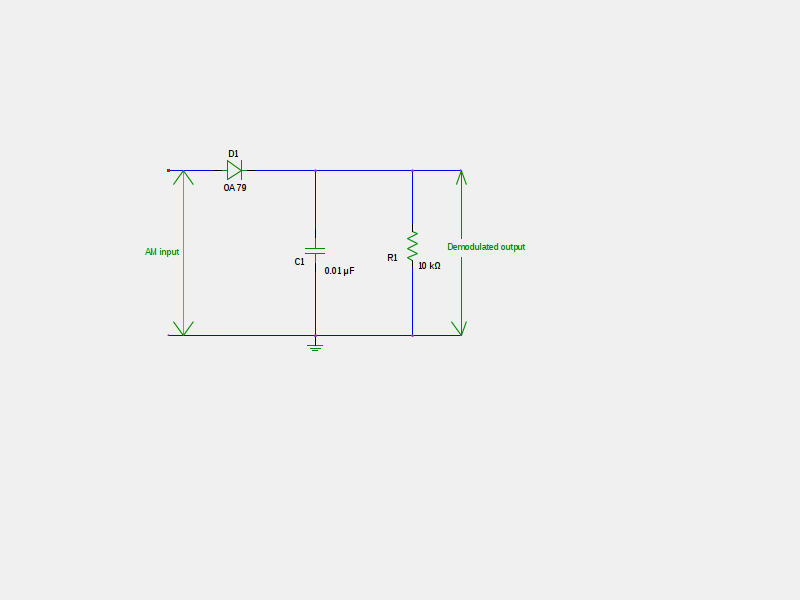
\includegraphics[width=15cm, height=10cm, trim=5cm 7.5cm 7.5cm 4cm, clip=true]{AMDemod.png}
\caption{AM Demodulation-Simple Diode Detector}
\label{AMDemod} 
\end{figure}
The circuit diagram for AM Demodulator using a simple diode detector is shown in Fig. \ref{AMDemod}.

\section*{Components and Equipments Required}
CRO, Function Generators(2), Breadboard, Probes.
\\Diodes- OA79
\\Capacitor- 0.01 $\mu$F
\\Resistor-10k$\Omega$
\section*{Procedure}

\begin{enumerate}
\item
Make connections on the breadboard as per the circuit diagram.
\item
Supply AM signal either from the signal generator or from the circuit designed in experiment Amplitude Modulation- Generation. 
\item
Connect the demodulated output to one channel of CRO along with the unmodulated signal on the other channel.
\item
Observe the Modulated and demodulated waveforms and plot it on a graph sheet.
\end{enumerate}
\section*{Observation}
A model plot showing the expected result of the experiment is shown in the Fig.\ref{AMdemod}
\begin{figure}
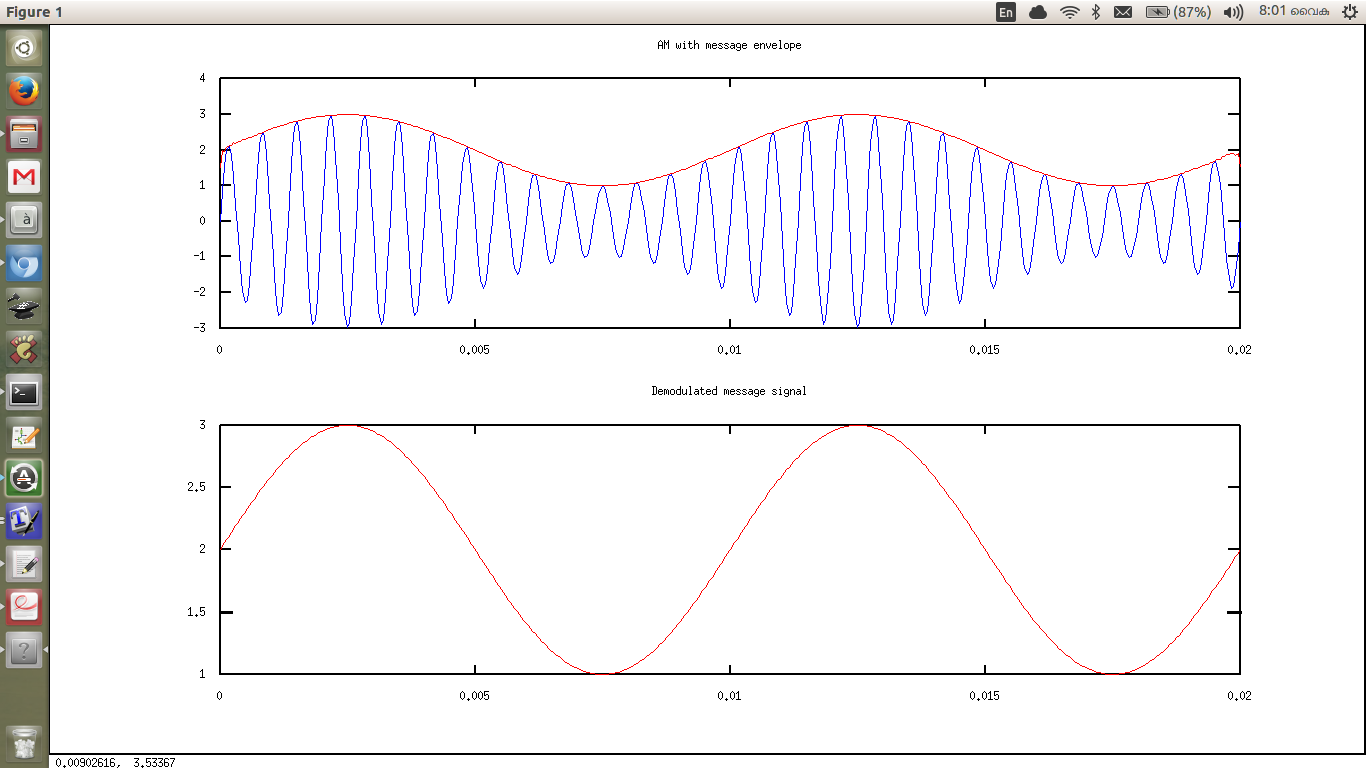
\includegraphics[width=12cm, height=10cm, trim= 2cm 1cm 1cm 1cm,clip=true]{AMdemod.png}
\caption{Modulated AM signal and Demodulated carrier}
\label{AMdemod}
\end{figure}

\section*{Result}

AM demodulation circuit was implemented on breadboard and output was observed and plotted ona graph sheet.

\chapter[AM Detection with Automatic Gain Control]{AM Detection with Automatic Gain Control}
\label{agcdetect}
\section*{Aim}
To demodulate the message content from AM signal. Also detect the automatic gain control signal from the received AM signal.
\section*{Theory}


A simple AM demodulator is a diode envelope detector.It can be implemented by a simple diode envelope detector to eliminate the negative half of the carrier envelope followed by a simple RC filter to remove the high frequency carrier. The result will be the low frequency envelope which is the demodulated message.

\paragraph{}
A diode with low junction capacitance is used in the circuit as it is has to rectify high frequency carrier.It offers low impedence at high frequency. The RC elements used at the output of the diode acts as a filter. Its time constant is chosen wisely so that it is too slow to follow the high frequency of the carrier wave at the same time its fast enough to follow the low frequency message envelope. 

The demodulated output voltage is having a modulating signal and a dc offset voltage. The dc offset voltage is proportional to the strength of the modulated signal received by the receiver in a transmission reception system, which inturn is proportional to the strength(amplitude) of the carrier.

\paragraph{Simple AGC:} From the detected output this dc voltage is separated by a LPF to get the required AGC feedback voltage. In superheterodyne receivers this AGC voltage is fed back to the IF amplifier stages of the receiver to increase or decrease the gain of the amplifier in such a way to get a constant output from the receiver.

\paragraph{Delayed AGC:}In simple AGC circuits even if the signal level received is low, the AGC circuit operates and the overall gain of the receiver is getting reduced. To avoid this situation, a delayed AGC circuit is used. In this case AGC bias voltage is not applied to amplifiers, until signal strength has reached a predetermined level after which AGC bias is applied like simple AGC.

\section*{Design}

 After the envelope detector, a properly designed low pass filter is added to filter out the high frequency carrier and to retain the low frequency modulating signal. This signal contains a dc level also which can be used for automatic Gain Control (AGC) for the IF amplifier stages of a superhetrodyne receiver.\\

\noindent Let the carrier frequency be $f_c=455\ kHz$ and maximum modulating signal frequency be $f_m=10\ kHz$

\noindent Inorder to design a lowpass filter with upper cutoff frequency 10 kHz,
\begin{equation}
f_H=\frac{1}{2\pi R_dC_d}
\end{equation}
\begin{equation}
10\ kHz=\frac{1}{2\pi R_dC_d}
\end{equation}
\noindent Select $C_d=\ 0.001 \mu F$. Then $R_d=\ 16.1k\Omega$.
Choose $R_d=\ 15k\Omega \ or\ 22k\Omega$ standard resistor values.\\

\noindent Make a $\pi$ filter using these $R_d$ and $C_d$ values. This completes the envelope detector part.
\paragraph{AGC Circuit:} The AGC lowpass filter $R_a$ and $C_a$ is seected in such a way as to eliminate full ac from the output and get a pure dc AGC voltage. 
Hence assuming a cutoff frequency of 10 Hz to eliminte the fluctuations,
\begin{equation}
10 Hz= \frac{1}{2\pi R_aC_a}
\end{equation}
\noindent Assuming $C_a=1 \mu F$, we get $R_a=15 k \Omega$
\paragraph{Delayed AGC Circuit:}
Here the simple AGC circuit is applied to a difference amplifier.  Delayed AGC output will be produced only when input voltage $V_i$ exceeds the threshold voltage which can be set to the desired value by adjusting the dc level of the potentiometer.

LM 741 opamp is chosen as the amplifying element. It is configured in difference amplifier mode. The Simple AGC volatge derived from previous 
circuit is used as the input to the inverting terminal of the  difference amplifier throgh the input resistance $R_i$. The threshold voltage is set at the non-inverting terminal. The voltage at non-inverting terminal can be varied in between +12V and 0V.

The gain of the difference volatage is determined by the values of feedback resistance $R_f$, input resistance $R_i$ and the position of variabale terminal of the potentiometer. The opamap is biased using +12V and -12 V respectively. 
The values of ristances are chosen as:

\begin{equation}
R_i\ =\ R_f\ =R_{pot}\ =100 k \Omega
\end{equation}
\section*{Circuit Diagram}
The detector circuit with simple AGC is shown in Fig. \ref{detectagcckt} and with delayed AGC is shown in Fig. \ref{delayedagcckt}.
\begin{figure}

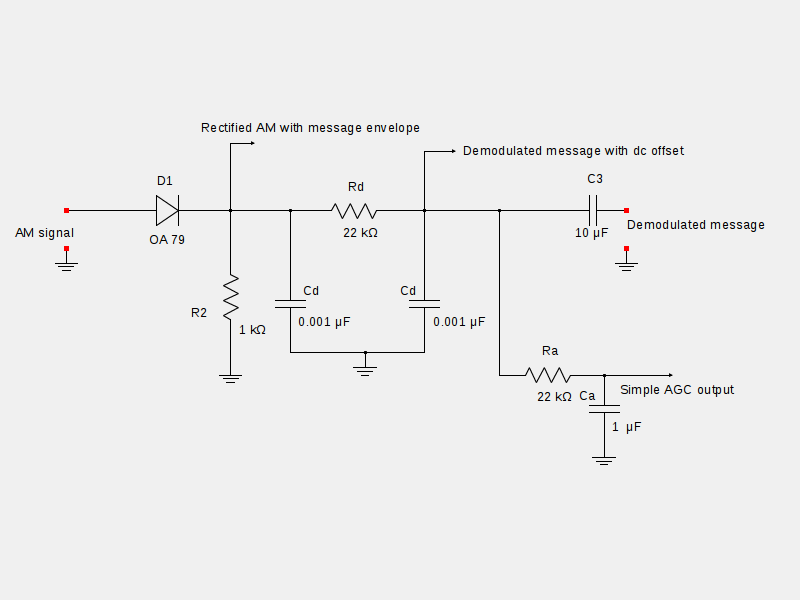
\includegraphics[height=8cm,width=15cm, trim=0cm 2cm 0cm 3cm,clip=true]{amdetectagc.png}
\caption{Detector circuit with Simple AGC}
\label{detectagcckt}
\end{figure}

\begin{figure}

\centering 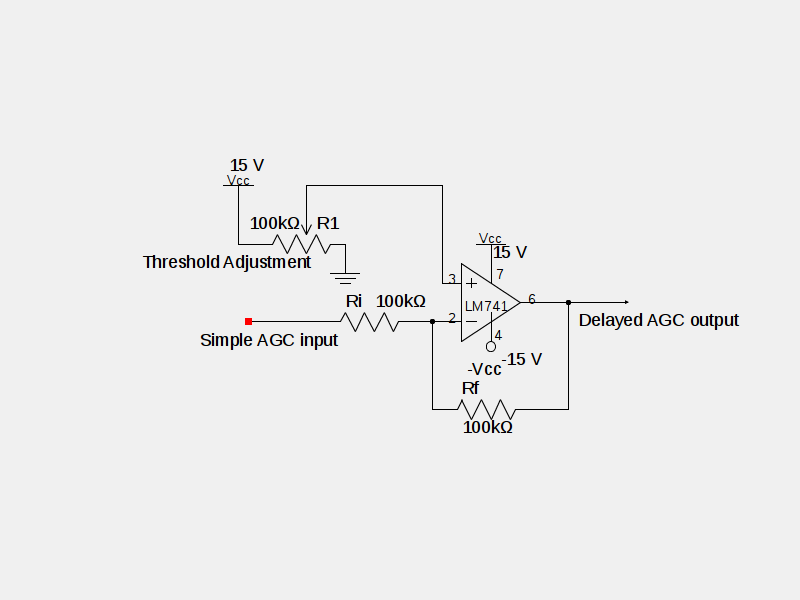
\includegraphics[height=8cm,width=12cm, trim=0cm 0cm 0cm 3cm,clip=true]{delayedagc.png}
\caption{Detector circuit for delayed AGC}
\label{delayedagcckt}
\end{figure}
\section*{Procedure}
\begin{enumerate}
\item
{Connect the diode to the output of AM signal as in the circuit diagram Fig. \ref{detectagcckt}.}
\item
Connect load resistance $R_L$ and observe the outputwaveform on a CRO and plot it.
\item
Connect the $\pi$ filter circuit of $R_d$ and $C_d$ and observe the output waveform on a CRO and plot it.
\item
Obtain the demodulated output without dc offset by connecting capacitor $C_3$. Observe it on a CRO and plot it.
\item
Connect the lowpass filter using $C_a$ and $R_a$ for obtaining AGC voltage level. Observe it on a CRO and plot it.
\item
Feed the AGC voltage to the delayed AGC	circuit of Fig. \ref{delayedagcckt}.
\item
Set the threshold to a fixed value, say $V_{threshold}=).5 V$. Keep the carier amplitude to the lowest, so that modulation index is 1.
\item
Slightly go on increasing the carrier amplitude. Note that for small values of carrier amplitude, delayed AGC voltage is positive. When it is above a certain limit the delayed AGC value becomes negative.
\end{enumerate}
\section*{Observation}
The following are the observed results of the experiment. See Fig. \ref{demodagcwaves}.
The threshod voltage for the signal level of carrier for which AGC starts applying is determined.
\begin{figure}
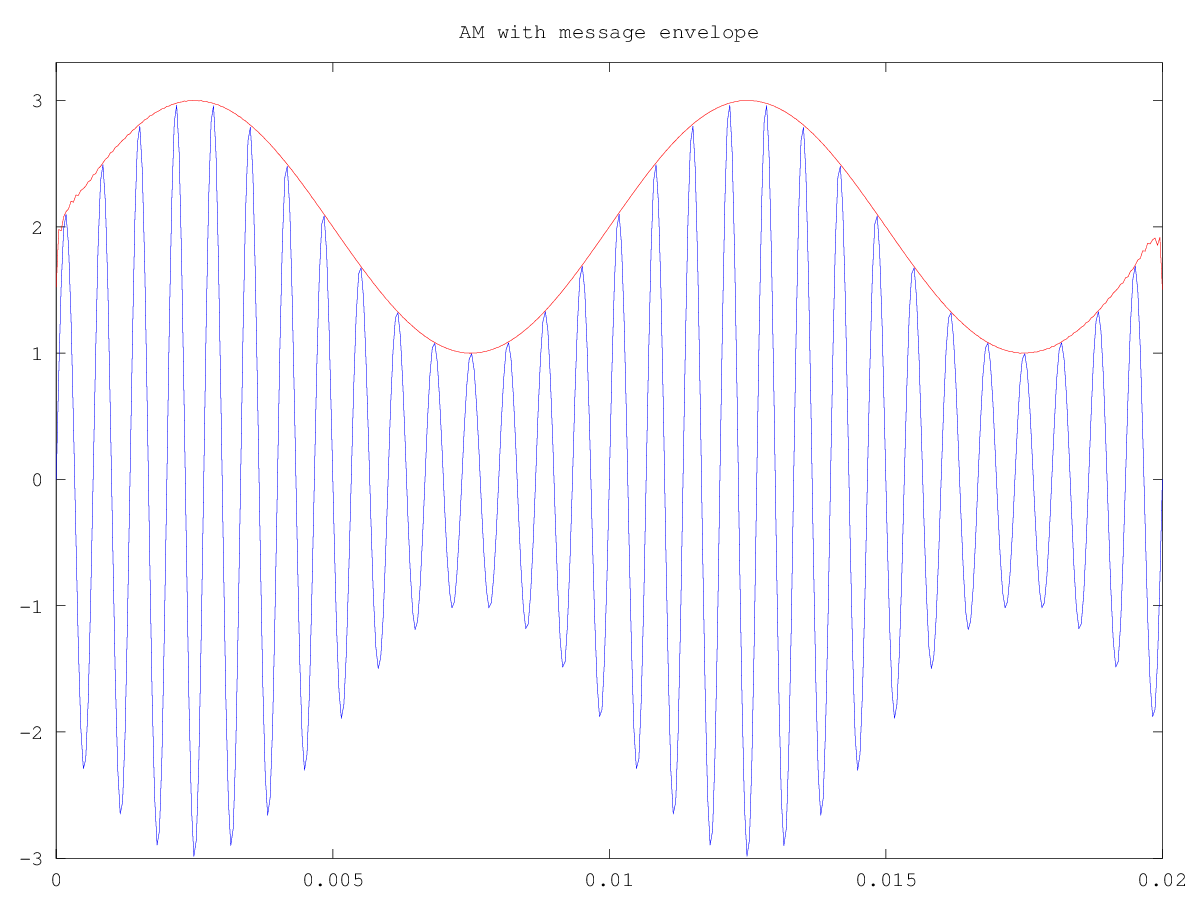
\includegraphics[height=4cm, width=12cm]{am.png}
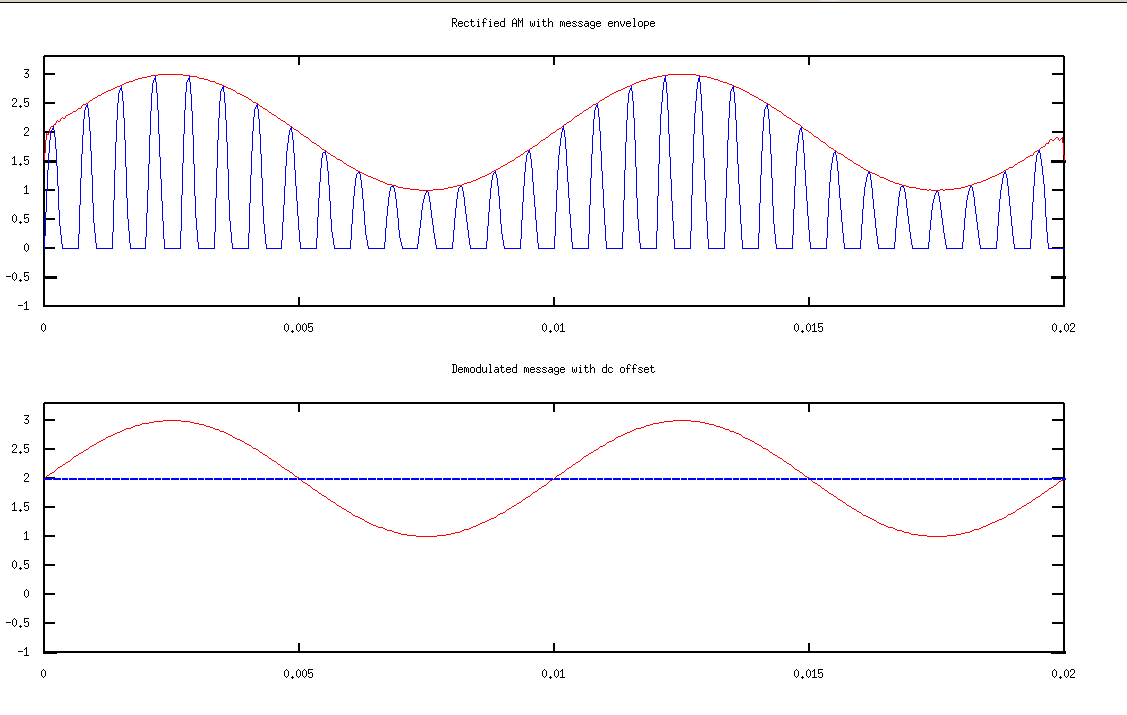
\includegraphics[height=7cm, width=12cm]{demodfig.png}
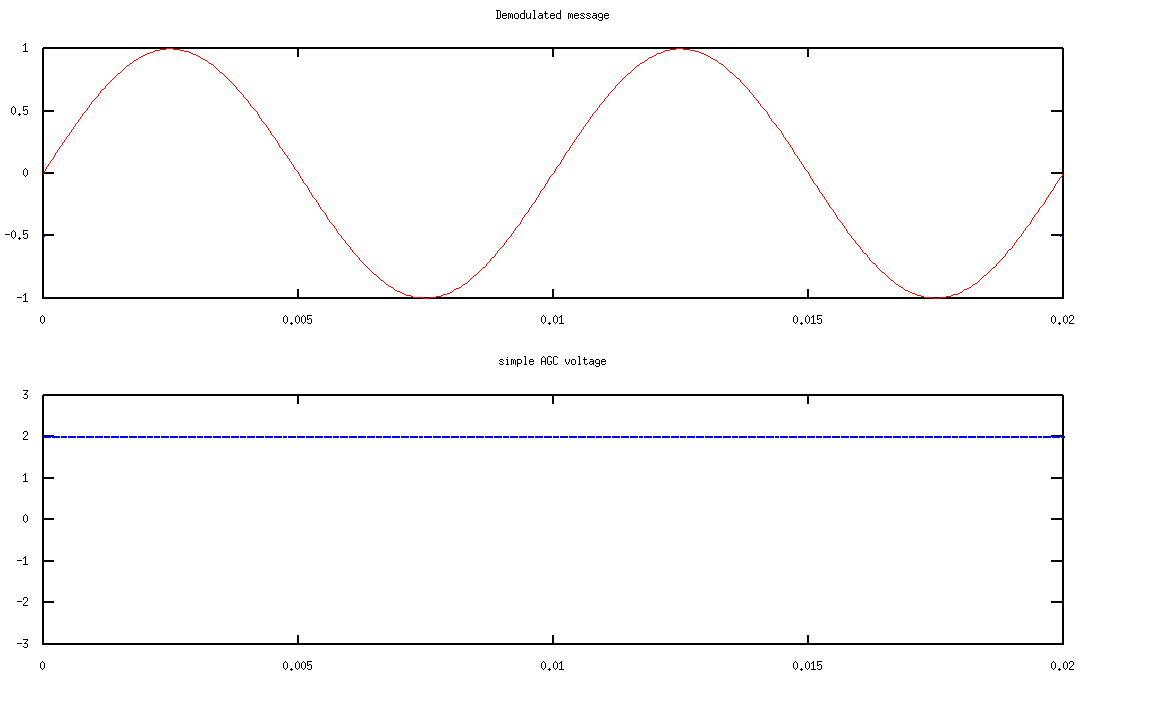
\includegraphics[height=7cm, width=12cm]{demodagc2.png}
\caption{Output waveforms from demodulation circuit}
\label{demodagcwaves}
\end{figure}

\section*{Result}

Demodulation circuit was designed and implemented with simple and delayed AGC.

\chapter[Mixer Circuit using BJT]{Mixer (Frequency Converter) Circuit using BJT}
\section*{Aim}
To design and set up a frequency converter circuit to produce an output frequency ($f_0$) which is the difference frequency between the two input frequency, ($f_{1}-f_{2}$).
\section*{Theory}
A mixer or frequency mixer is a nonlinear electrical circuit that creates new frequencies from two signals applied to it. In its most common application, two signals at frequencies $f_1$ and $f_2$ are applied to a mixer, and it produces new signals at the sum $f_1 + f_2$ and difference $f_1 - f_2$ of the original frequencies. Other frequency components (like $f_1 \pm 2f_2$ may also be produced in a practical frequency mixer.\footnote{\url{http://en.wikipedia.org/wiki/Frequency_mixer}}

The most important application of mixers are in superhetrodyne receivers where the very high carrier frequency is down converted to an intermediate frequency. This is done by mixing the carrier frequency with a locally generated oscillator frequency to get an output frequency which is the difference between local oscillator frequency and incoming signal frequency, ie the intermediate frequency. In widely used AM receivers the local oscillator frequency is so chosen with respect to carrier frequency such that their difference is a constsnt intermediate frequency of 455kHz.\\
\begin{center}
$f_{IF}=f_{oscillator}-f_{carrier}=455 kHz$
\end{center}
The mixer output which contains all image frequencies of $f_1 \pm nf_2$ is filtered to obtain the required difference frequency $f_1-f_2$.
\section*{Design}
Let the input at the base be 10kHz($f_1$) signal and at the emitter be 9 kHz($f_2$) signal such that the output contains their sum and difference frequencies. The output can be low pass filtered to obtain the difference frequency $f_1-f_2=1 \ KHz$.
\\ Choose Transistor BC107. See \ref{BC107} for its datasheet details. 
\noindent Take $V_{CC}=12 V$ and $I_C=2 mA$ under dc biasing conditions.

\noindent For Class A mode of operation, let
\begin{equation}
V_{CE}=\ 50\% \ of V_{CC}=\ 6 V
\end{equation}
\begin{equation}
V_{RC}=\ 40\% \ of V_{CC}=\ 4.8 V
\end{equation}
\begin{equation}
V_{RE}=\ 10\% \ of V_{CC}=\ 1.2 V
\end{equation}

 \paragraph{Design of Emitter and Collector Resistors}
 
\begin{equation}
R_C=\ \frac{V_{RC}}{I_C}=\ \frac{4.8V}{2mA}=\ 2.4 k \Omega. \approx 2.2k\Omega (\ standard \ resistor\  value)
\end{equation}
\begin{equation}
R_E=\ \frac{V_{RE}}{I_E}=\ \frac{1.2V}{2mA}=\ 600 \Omega. \approx 560\Omega (\ standard \ resistor \ value)
\end{equation}
\noindent (Since $I_C \approx I_E =2mA$)

\paragraph{Design of Potential divider resistors $R_1$ and $R_2$ \\}
\noindent At dc bias point,
\begin{equation}
I_B=\ \frac{I_C}{h_{fEmin}}=\ \frac{2mA}{110} \approx 20 \mu A
\end{equation}

\noindent Let the current through $R_1$ be $10I_B$ and that through $R_2$ be $9I_B$ such that $I_B$ flows through the base of BC107.
\begin{equation}
I_{R1}=\ 10I_B=\ 200 \mu A
\end{equation}
\begin{equation}
I_{R2}=\ 9I_B=\ 180 \mu A
\end{equation}



\noindent Voltage across resistor $R_2$ is,
\begin{equation}
V_{R2}= V_{RE} +V_{BEactive} =\ 1.2V+0.6V=\ 1.8 V
\end{equation}
 \begin{equation}
R_2=\ \frac{V_{R2}}{I_2}= \ \frac{1.8V}{180 \mu A}=\ 100k\Omega
\end{equation}

\noindent Voltage across resistor $R_1$ is,
\begin{equation}
V_{R1}= V_{CC} +V_{R2} =\ 12V-1.8V=\ 10.2 V
\end{equation}
 \begin{equation}
R_1=\ \frac{V_{R1}}{I_1}= \ \frac{10.2V}{200 \mu A}=\ 51k\Omega \approx 47 k\Omega (\ standard \ resistor \ value)
\end{equation}

\paragraph{Design of coupling capaciors\\}
\noindent $C_1 = 1 \mu F$ and $C_E = 0.1 \mu F $

\paragraph{Design of Filter Circuit\\}

\noindent Inorder to lowpass filter the output signal choose the upper cut-off frequency be $f_o$=1.5kHz so that the required output 1 kHz appears in the pass band.
\noindent The cut-off frequency of lowpass filter is,
\begin{equation}
f_o=\ \frac{1}{2\pi R_fC_f}=1.5\ kHz
\end{equation}
\noindent where $R_f$ and $C_f$ are the passive filter components.

Choose $R_f=\ 10k\Omega$
\begin{equation}
\therefore C_f=\frac{1}{2\pi R_f f_o} \approx 0.01 \mu F.
\end{equation}
\noindent Choose $\pi$ filter configuration for better performance.
\section*{Components and Equipments required}
Function Generators(2), CRO(1), Connection wires, Breadboard, Probes.
\\BC107 (1)
\\ $47k\Omega,\  10k\Omega\ (2),\ 560\Omega,\,\ 2.2k\Omega ,\ 10k\Omega (2) $- Resistors
\\ $ 1\mu F (1),\ 0.1\mu F (1), \ 0.01\mu F (3)$ - Capacitor
\section*{Circuit Diagram}
See Figure \ref{mixer} for circuit diagram.
\begin{figure}[h]
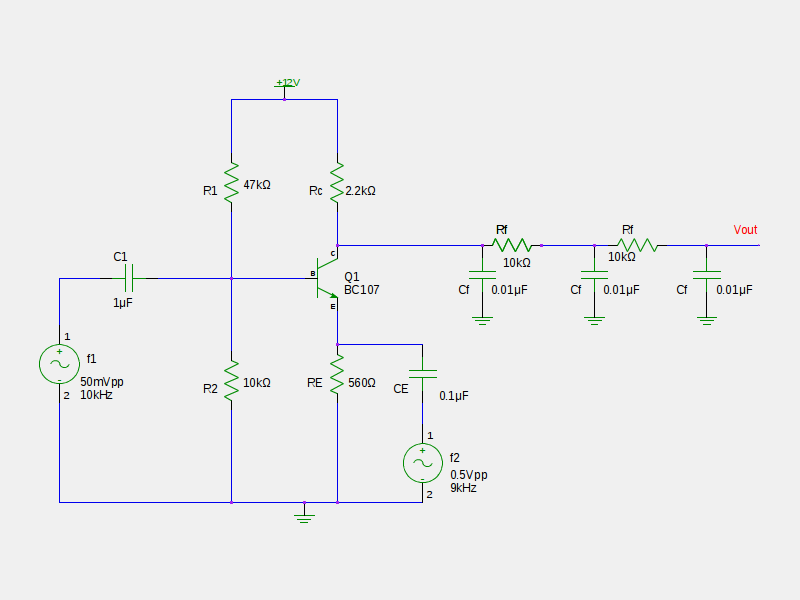
\includegraphics[width=\textwidth, height=10cm, trim=3cm 3cm 3cm 3cm,clip=true]{mixer.png}
\caption{Circuit Diagram for Mixer circuit using BJT}
\label{mixer}
\end{figure}
\section*{Procedure}
\begin{enumerate}
\item
Make connections as per the circuit diagram.
\item
Feed $f_1$ and $f_2$ with amplitudes as shown in the circuit diagram and frequencies 10 kHz and 9 kHz respectively.
\item
Observe the filtered output frequency on a CRO.
\item
Repeat with frequencies changed to 20 kHz and 19kHz  (50 kHz and 49 kHz)and observe it in CRO. Verify that the circuit gives the difference frequency of 1 kHz at the output.
\item
Plot the input and output signals on a graph sheet. 

\end{enumerate}
\section*{Observation}
From the graph find the frequency of the output signal.\\
\textcolor{red}{Model graph to be added}
\section*{Result}
The mixer circuit using BJT was set up and output was verified from signals observed on a CRO.



\chapter[DSB-SC using multiplier IC AD633]{DSB-SC using multiplier IC AD633}
\label{chapdsbsc}
\section*{Aim}
To set up a balanced modulator circuit for double side band suppressed carrier amplitude modulator.To implement a demodulator to obtain the message signal.
\section*{Theory}
DSB-SC is a kind of amplitude modulation in which the carrier frequency component is absent. It is generated by multiplying the carrier and modulating signals. If $e_c$ is the carrier and $e_m$is the message signal, where
\begin{equation}
e_c=E_c\  sin\ 2\pi f_ct
\end{equation}
\begin{equation}
e_m=E_m\  sin\ 2\pi f_mt
\end{equation}
Multiplication is done using AD633 (See \ref{AD633}) multiplier IC.
Applying $e_m$ to $\textbf{X}$ and $e_c$ to $\textbf{Y}$ with $\textbf{Z}$ grounded, 
\begin{equation}
W= \frac{e_me_c}{10} =\frac{Emsin(2\pi f_mt).Ecsin(2\pi f_ct)}{10}
\end{equation}
\begin{equation}
W= \frac{E_mE_c}{10} \frac{[cos 2\pi (f_c\ -\ f_m)t-cos 2\pi (f_c\ +\ f_m)t]}{2}
\end{equation}
\begin{equation}
W= \frac{E_mE_c [cos 2\pi (f_c\ -\ f_m)t]}{20}- \frac{E_mE_c[cos 2\pi (f_c\ +\ f_m)t]}{20}
\end{equation}
This wave contains both the sidebands at $f_c-f_m$ and $f_c+f_m$, but not the wave at carrier frequency\footnote{$sin \ A.\ sin\ B=\frac{cos\ (A-B)-cos\ (A+B)}{2}$}. Hence the name double sideband suppressed carrier modulation(DSB-SC).

The following figure \ref{DSBSC} shows\footnote{Image Courtesy: \href{http://commons.wikimedia.org/wiki/File\%3AAM-DSBSC.png}{Serych at cs.wikipedia [Public domain], from Wikimedia Commons}} the DSB-SC signal in blue and the original message is shown in red. (\emph{It is an indicative graph, not to scale as per the experimental set-up.})
\begin{figure}[h]
\begin{center}
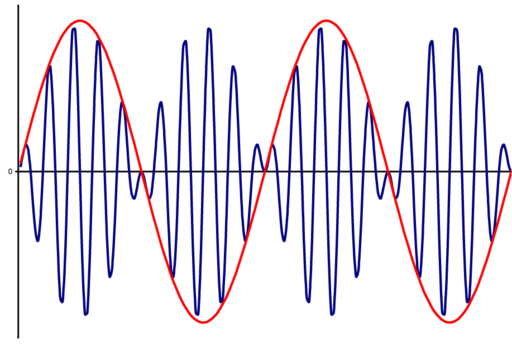
\includegraphics[width=10cm,height=4cm]{AMDSBSC.png}
\caption{DSB-SC signal in blue, original message shown in red.}
\label{DSBSC}
\end{center}

\end{figure}

Multiplying the DSB-SC with the carrier once again will result in the following output.
\begin{equation}
\begin{split}
W=\frac{1}{10} &[ \frac{E_mE_c [cos (2\pi (f_c\ -\ f_m)t)]}{20} \\
&\quad -\frac{E_mE_c[cos (2\pi (f_c\ +\ f_m)t)]}{20}].
 E_c sin(2\pi f_ct)
\end{split}
\end{equation}

\begin{equation}
\begin{split}
W=& \frac{E_m.{E_c}^2}{400}sin(2\pi (2f_c-f_m)t)  -  \frac{E_m.{E_c}^2}{400}sin(2\pi (2f_c+f_m)t)\\ 
&\quad +\frac{E_m.{E_c}^2}{200}sin(2\pi f_mt)
\end{split}
\end{equation}
Thus the signal consists of various frequencies of which, the smallest is the message frequency. It can be extracted by filtering using a low pass filter. Since the amplitude of the message frequency is very small, It may be amplified using a simple non-inverting amplifier using an opamp.

%%%%%%%%%%%%%%%%%%%%%%%%%%%%%%%%%%%
\begin{figure}[ht]
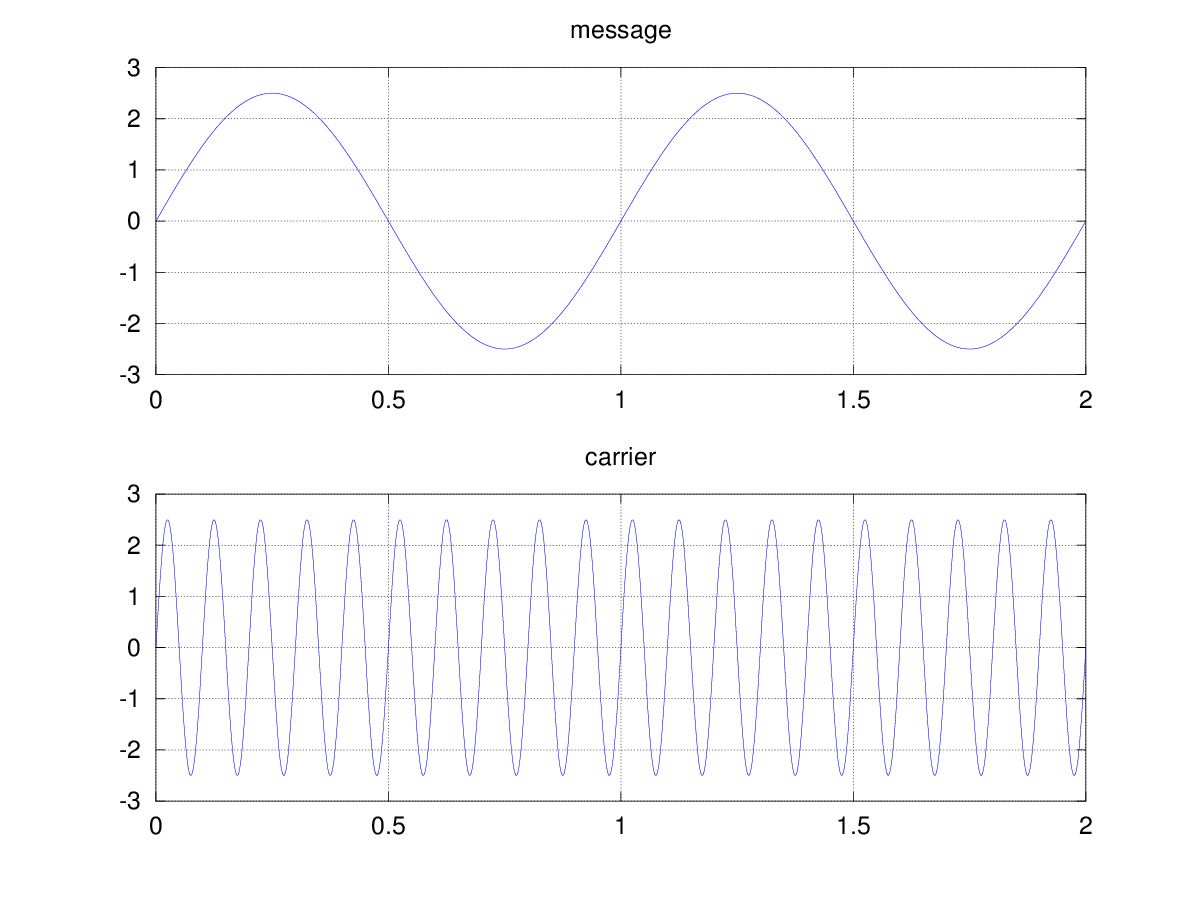
\includegraphics[width=\textwidth]{am6331.png}
\caption{Message and carrier signals}
\label{msg633plot1}
\end{figure}
%%%%%%%%%%%%%%%%%%%%%%%%%%%%%%%%%%%%
\section*{Design}

To the \textbf{X} input of the IC, feed the message sinusoid of amplitude $E_m=2.5\ V$ (ie., peak to peak amplitude of 5 V) and frequency $f_m= 1\ kHz$.\\

To the \textbf{Y} input of the IC, feed the carrier sinusoid of amplitude $E_c=2.5\ V$ and frequency $f_c= 100\ kHz$.\\
Ground the \textbf{Z} input of the IC.\\
Provide the supply voltage of \textbf{+15 V to pin 8} of the IC and \textbf{-15 V to pin 5} of the IC.\\

The output signal will have a waveform as given by,

\begin{equation}
W=\frac{X.Y}{10}+Z
\end{equation}
\begin{equation}
W=\frac{e_m.e_c}{10}=\frac{(2.5) \ .(2.5)}{10}\frac{[cos 2\pi99kt-cos 2\pi101kt]}{2}
\end{equation}

\begin{equation}
W=\frac{6.25}{20}[cos 2\pi99kt-cos 2\pi101kt]
\end{equation}

 This is the DSB-SC waveform.
 
 \begin{figure}[ht]
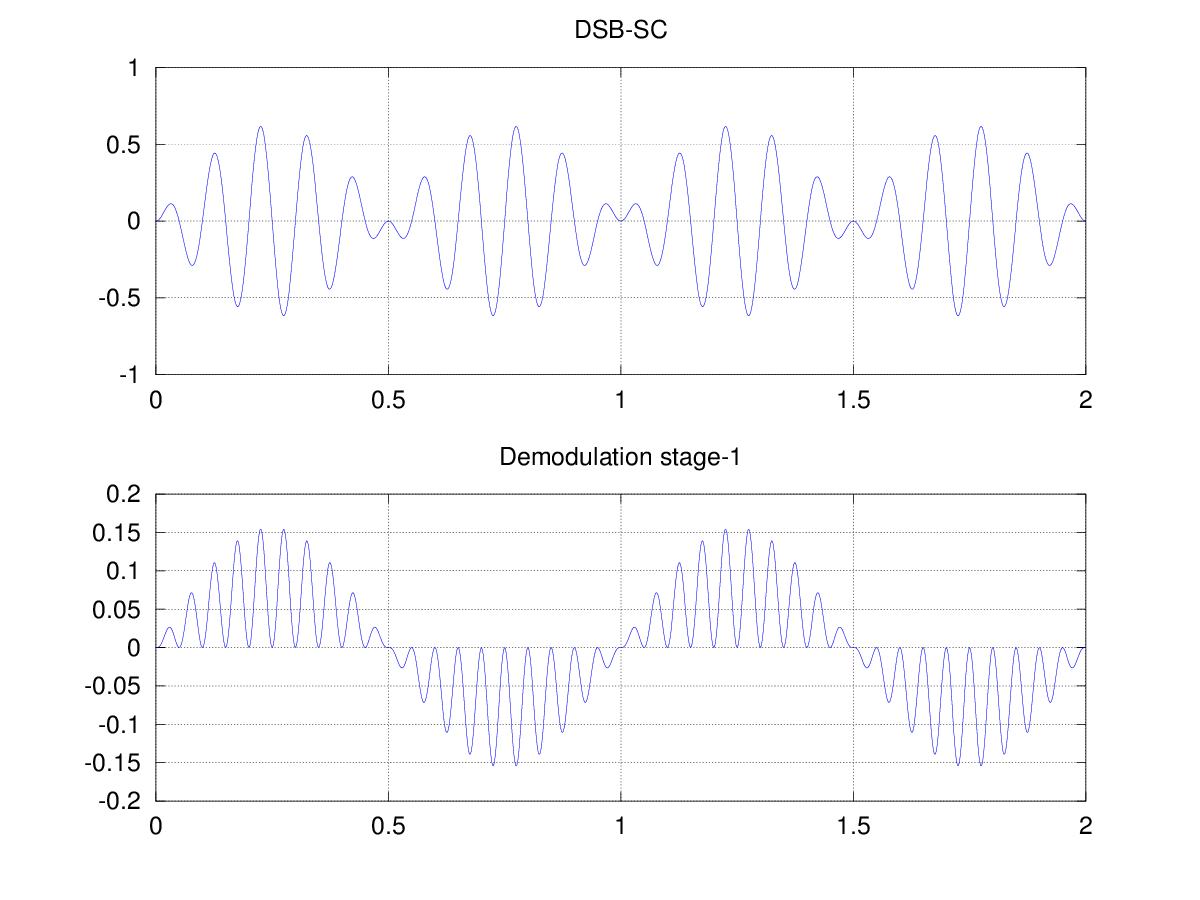
\includegraphics[width=\textwidth]{dsbsc6332.png}
\caption{AM(DSB-FC) and Demodulation stage-1 signals}
\label{dsbsc633plot2}
\end{figure}
 
 \paragraph{Demodulation}  is by multiplying the DSB-SC signal once again with the carrier. This can be implemented by connecting another AD633 IC in cascade with the first one.

\noindent The multiplication will result in the following output, as per the theory already explained.

\begin{equation}
\begin{split}
W=& \frac{15.625}{200}sin(2\pi 1kt)\\
&\quad  +\frac{15.625}{400}sin(2\pi199kt) -\frac{15.625}{400}sin(2\pi 201kt)
\end{split}
\end{equation}

\noindent This waveform is shown in Figure \ref{dsbsc633plot2}, which is the stage -1 in demodulation. The next step is to obtain the message signal. This is done by lowpass filtering the above signal at a cut-off frequency of 1.5 kHz.

To design an RC lowpass filter of cut-off frequency 1.5 kHz,

\begin{equation}
f_c=\frac{1}{2\pi R_1C_1}=1.5kHz
\end{equation}
Choose $C_1=0.01\  \mu F$
$\therefore  R_1 =10 \ k \Omega$

A non-inverting amplifier may be used to amplify this signal. Using a feedback resistor of $R_f= 100 \ \k \Omega$ and an input resistance of $R_i=10\ k\Omega$ will result in a gain of $A_v=1+\frac{R_f}{R_i}=11$.
\begin{sidewaysfigure}[ht]
    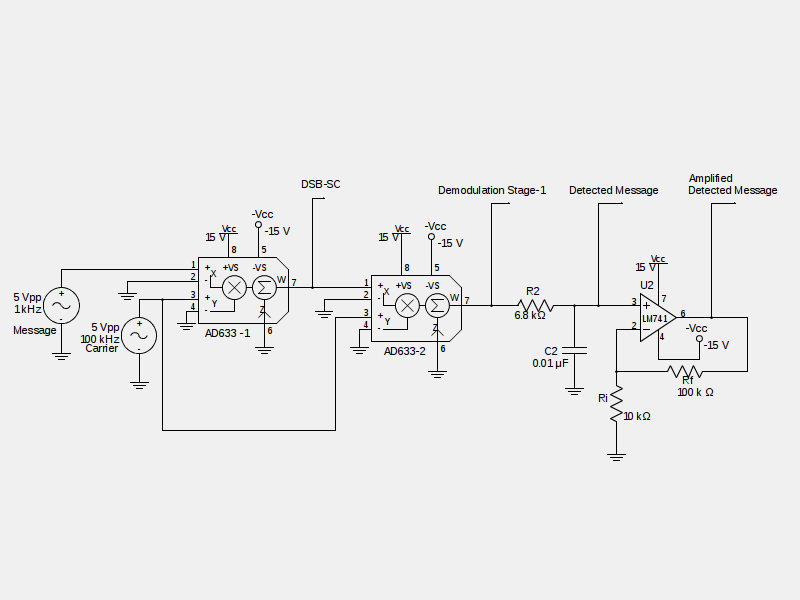
\includegraphics[scale=0.8, trim=0cm 4cm 0cm 4cm,clip=true]{633dsbsc.png}
    \caption{Circuit for DSB-SC generation and detection using AD633 multiplier IC}
    \label{DSBSCckt}
\end{sidewaysfigure}


\section*{Circuit Diagram}
The circuit diagram for implementing DSBSC using multiplier IC is shown in figure \ref{DSBSCckt}.




\section*{Procedure}
\begin{itemize}
\item
Make connections as shown in the circuit diagram, figure \ref{DSBSCckt}.
\item
Feed the message and carrier signals.
\item
Connect the pin number 7 of the IC to a CRO and observe the resultant waveform which is DSB-SC.
\item
Connect the pin number 7 of the second IC to a CRO and observe the resultant waveform which is the product of DSB-SC and the carrier.(Named demodulation stage-1 signal)
\item
Observe the output from the filter, amplified by the opamp amplifier, which extracts the envelope -\emph{The 1kHz message signal}- of the previous signal.
\item
Plot the signals observed on a graph sheet.
\end{itemize}
\section*{Observation}



The input and output signals as observed on a CRO are shown in Figure \ref{msg633plot1} and \ref{dsbsc633plot2}.


\section*{Result}
Implemented DSB-SC using multiplier IC AD 633 and observed the signal waveforms.
\chapter[FM generation - Reactance Modulator]{FM generation - Reactance Modulator}
\section*{Aim}
\section*{Theory}
\section*{Design}
\section*{Circuit Diagram}
\section*{Procedure}
\section*{Observation}
\section*{Result}
\chapter[FM Demodulation]{FM Demodulation}
\section*{Aim}
\section*{Theory}
\section*{Design}
\section*{Circuit Diagram}
\section*{Procedure}
\section*{Observation}
\section*{Result}
\chapter[PAM Generation and Demodulation]{PAM Generation and Demodulation}

\section*{Aim}
To set-up and implement circuits to carry out pulse amplitude modulation. To design demodulationg circuits to detect the message from pulse amplitude modulated wave.
\section*{Theory}
Pulse amplitude modulation is a kind of digital modulation technique in which analog message signal is sampled at constant frequency - \emph{carrier frequency}. A pulse of specified duration is used to sample the message signal. When the pulse is on, the message is sampled and when it is off no message is sampled. This is a basic step in the digitization of analog message signals. The circuits to be implemented in this experiment does a kind of natural sampling.\footnote{For more on natural sampling, refer Digital Transmission \cite{Tomasi}}.

Waveforms showing pulse carriers whose amplitude is modulated buy message is shown in Figure \ref{PAMmod1} and \ref{PAMmod2}. A simple way to implement this is to allow the message to be fed as the input to a switch and the switch ON/OFF time is controlled by the pulses at sampling frequency.

The demodulation of PAM waveform can be implemented by using a lowpass filter which passes message signal frequenies but blocks the carrier signal.
\begin{figure}[h]
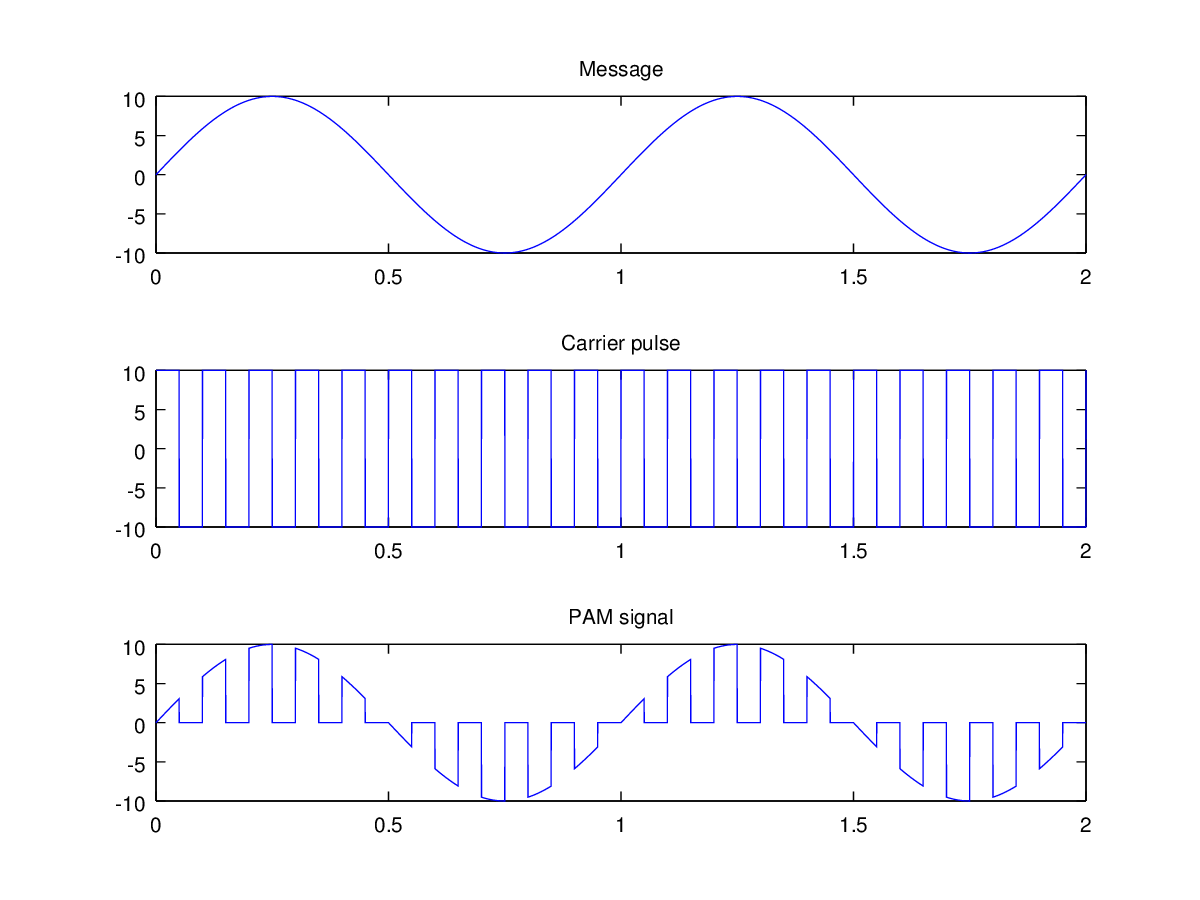
\includegraphics[width=\textwidth]{pam1.png}
\caption{PAM modulation using transistor}
\label{PAMmod1}
\end{figure}

\begin{figure}[h]
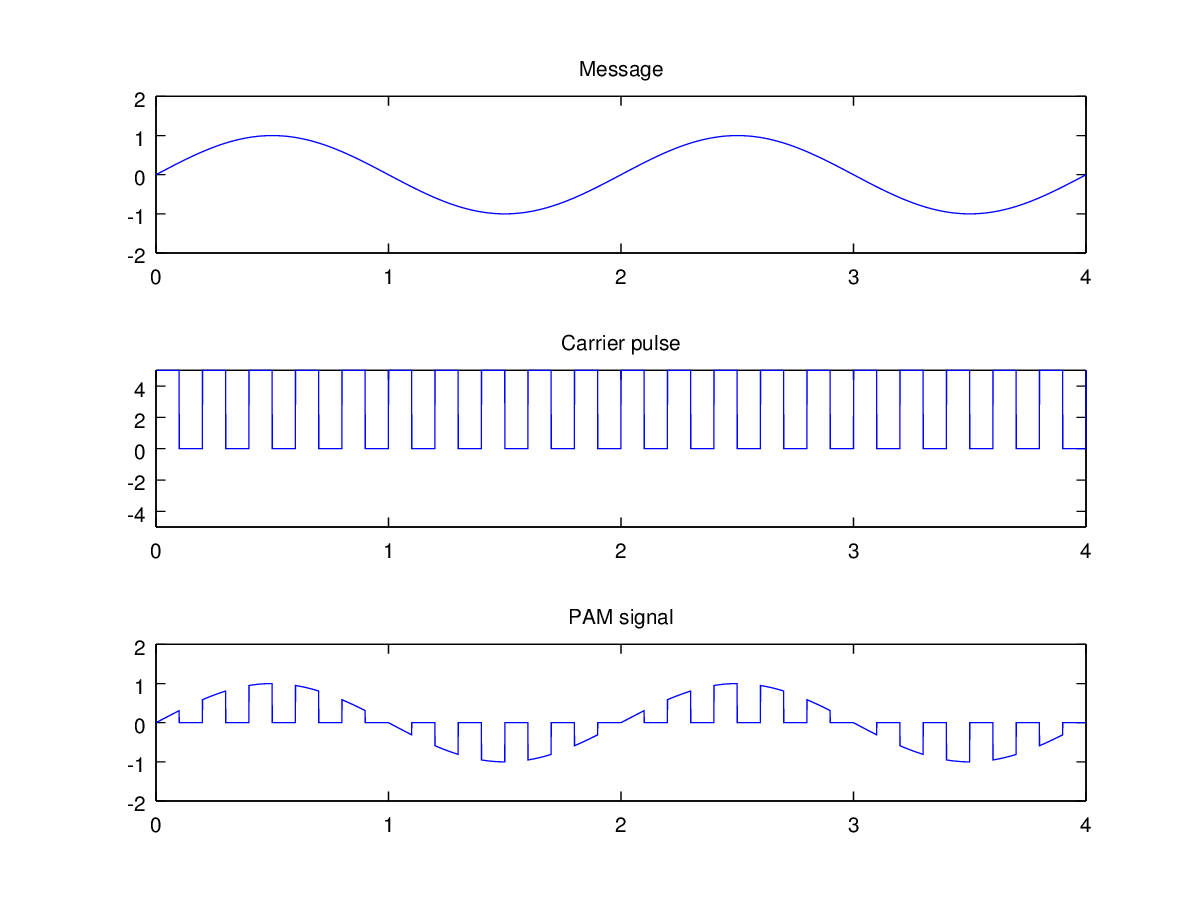
\includegraphics[width=\textwidth]{pam2.png}
\caption{PAM modulation using switching IC}
\label{PAMmod2}
\end{figure}
\section*{Design}
\subsection*{PAM using transistor as a switch}
One technique to implement PAM is to use transistr in switching mode. The flow of current from collector to emitter in a bipolar junction transistor is controlled by the voltage at its base. 


\noindent Choose the transistor BC107. For more details on BC107 see \ref{BC107}.
\noindent Apply the sinusoidal message signal of frequency $f_m < \ 1 \ kHz$ and amplitude $E_m<\ 10\ V_{pp}$ at the collector.
\noindent Apply a carrier at the transistor base through a resistor $10 k\Omega$. The carrier pulse amplitude is set as $E_c =10 \ V_{pp}$ and frequency $f_c=\ 10 kHz$.

\subsection*{PAM using CMOS switching IC CD4016}
CD 4016 is a quad bilateral CMOS switching IC. See \ref{4016} for more deatails. The message signal is fed to any of the input terminals of the switch and the modulating pulse carrier is fed as the control signal for the switch. The PAM output will be available at the output terminal of the switch which is fed to the CRO across a load resistor of $10\ k\Omega$. Keep the message signal frequency to be $f_m=500 \ Hz$ and the switching pulse of 10 kHz which is the carrier is to be fed  from the TTL output from a function generator.

\subsection*{Demodulation}
Demodulation is done using a  $\pi$ RC filter.
\noindent Design the filter as per the equation for upper cut-off frequency of a low pass filter,
\begin{equation}
f_H=\frac{1}{2\pi R_dC_d}
\end{equation}
\begin{equation}
1.5\ kHz=\frac{1}{2\pi R_dC_d}
\end{equation}
\noindent Select $C_d=\ 0.01 \mu F$. Then $R_d=\ 10k\Omega$.
Choose $R_d=\ 10k\Omega$ standard resistor value.\\

\section*{Circuit Diagram}
\subsection*{Using transistor as a switch}

The PAM generation using transistor as a switch and demodulation circuit is shown in Figure. \ref{pamckt}.

\begin{figure}
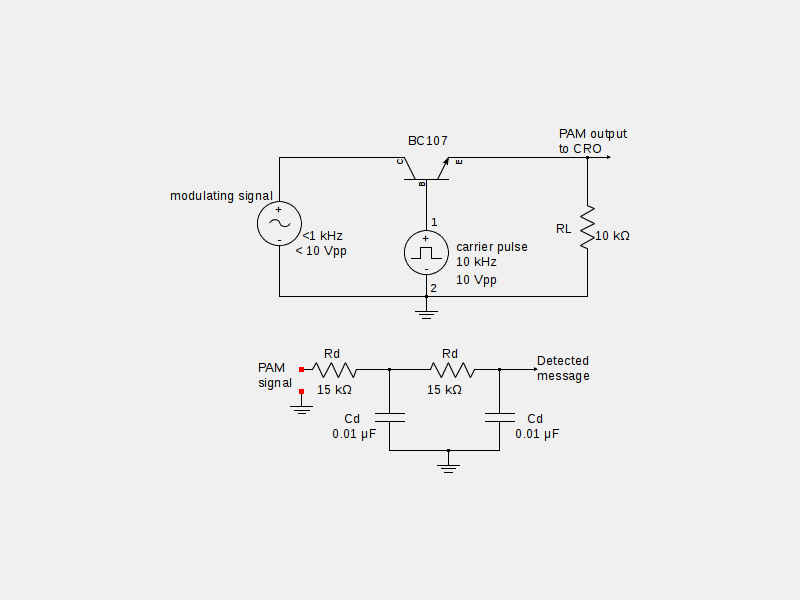
\includegraphics[width=\textwidth, trim=5cm 3cm 4cm 4cm,clip=true]{pamckt1.png}
\caption{PAM generation and demodulation circuuit}
\label{pamckt}
\end{figure}



\subsection*{Using CMOS switching IC CD4016}
The PAM generation using CD4016 is shown in Figure. \ref{pamckt2}. Demodulation can be done in the same way as shown in \ref{pamckt}.

\begin{figure}
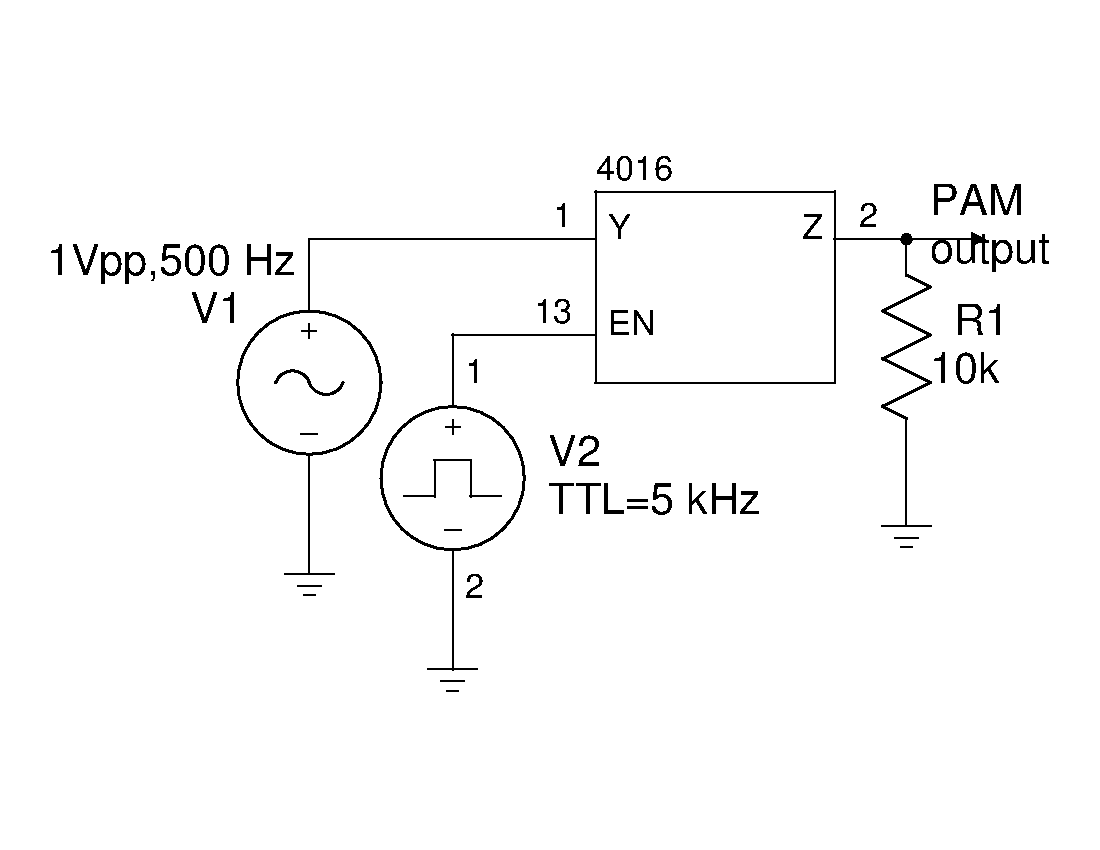
\includegraphics[width=\textwidth, height=7cm]{pamckt2.jpg}
\caption{PAM generation using CD4016}
\label{pamckt2}
\end{figure}

%\section*{Components and Equipments Required}
%CRO (1), \\Signal generator(2),
%\\Resistors: $15\ k\Omega$(2), $10\ k\Omega$(1)
%\\Capacitors: $0.01\  \mu F$(2)
\section*{Procedure}
\begin{itemize}
\item
Connect the PAM generating circuit as shown in the circuit diagram, Figure \ref{pamckt}.
\item
Feed the modulating message signal and the carrier pulses from the function generator.
\item
Observe the output on a CRO and plot the graphs of the input and output waveforms.
\item
Make the demodulating circuit as shown in the circuit diagram, Figure \ref{pamckt}.
\item
Repeat the PAM experiment using CD4016 IC.
\item
Make connections as shown in the circuit diagram Figure. \ref{pamckt2}. If IC is used for modulation make sure it is biased with $V_{DD}=5V$ and is properly grounded.
\item
Observe the input and output waveforms from PAM generaton and demodulation circuits using CD4016 IC.

\end{itemize}
\section*{Observation}
Plot the graphs of input and ou
tput waveforms as observed on a CRO.
\section*{Result}

Implemented the PAM generation and demodulation circuits using BJT as well as switching IC.



\chapter[FM Demodulation using PLL]{FM Demodulation using PLL}
\section*{Aim}
\section*{Theory}
\section*{Design}
\section*{Circuit Diagram}
\section*{Procedure}
\section*{Observation}
\section*{Result}

\chapter[AM generation and Demodulation]{AM generation and Demodulation}
\section*{Aim}
\section*{Theory}
\section*{Design}
\section*{Circuit Diagram}
\section*{Procedure}
\section*{Observation}
\section*{Result}
\chapter[SSB generation and Demodulation]{SSB generation and Demodulation}
\section*{Aim}
\section*{Theory}
\section*{Design}
\section*{Circuit Diagram}
\section*{Procedure}
\section*{Observation}
\section*{Result}
\begin{appendix}
\chapter {Quick Reference-Data on Components}
\section{BJT BF194/195}
\label{BF194/195}
BF194/195 is a high frequency transistor. From its datasheet 

Type Designator: BF194/BF195

Material of transistor: Si

Polarity: NPN

Maximum collector power dissipation ($Pc$), W: 0.25

Maximum collector-base voltage |$V_{cb}$|, V: 30

Maximum collector-emitter voltage |$V_{ce}$|, V: 20

Maximum emitter-base voltage |$V_{eb}$|, V: 5

Maximum collector current |$I_{c max}$|, mA: 30

Forward current transfer ratio (hFE), min: 67

\textcolor{red}{TODO: Pinout diagram to be added}
\section{BJT BC107}
\label{BC107}
Type Designator: BC107

Material of transistor: Si

Polarity: NPN

Maximum collector power dissipation ($P_c$), W: 0.3

Maximum collector-base voltage |$V_{cb}$|, V: 50

Maximum collector-emitter voltage |$V_{ce}$|, V: 45

Maximum emitter-base voltage |$V_{eb}$|, V: 6

Maximum collector current |$I_{cmax}$|, A: 0.1

Forward current transfer ratio ($h_{FE}$), min: 110

Package of BC107 transistor: TO18
\textcolor{red}{TODO: add schematic diagram and photo of BC107}

\section{Intermediate Frequency Transformer}
\label{IFT}
IFT act as parallel resonant circuits whose resonating frequency is around 455 kHz. This frequecy is adjustable by a factor of  \textcolor{red}{FIXME} plusorminus 10\%. IFT has a tappedd primary winding and a secondary winding. Primary winding has a capacitor connected in parallel internally. Its inductor value is $L_eq=450\ mu H$ and capacitance $C=270\ pF$. 
\\Its resonant frequency is thus $f=\frac{2\pi}{\sqrt{L_{eq}C}}\approx 455 kHz$.

\textcolor{red}{TODO: add schematic diagram and photo of IFT}
\end{appendix}
\begin{thebibliography}{1}
\bibitem{ACmanual}{LABORATORY MANUAL COMMUNICATIONS LABORATORYEE 321, CALIFORNIA STATE UNIVERSITY, LOS ANGELES
Lab-Volt Systems, Inc}

\end{thebibliography}


\end{document}
